\chapter{Viabilidad Comercial}

El presente capítulo tiene como objetivo analizar la viabilidad comercial de un teclado customizado de alta gama, diseñado específicamente para satisfacer las necesidades del mercado español. Este teclado se distingue por varias características innovadoras, incluyendo un diseño sin plate, la incorporación de una pantalla OLED, una conectividad Bluetooth y la disposición 105 ISO español, lo que lo convierte en una opción única en el mercado.

La viabilidad comercial de un producto no solo depende de su diseño y funcionalidad, sino también de una serie de factores que abarcan desde el análisis del mercado hasta los costos asociados con su producción y comercialización. En este capítulo, se llevará a cabo un análisis exhaustivo que abarca diversos aspectos cruciales para determinar la potencial aceptación y éxito del teclado en el mercado.

Primero, se realizará un análisis del proyecto, donde se evaluarán los objetivos, la propuesta de valor y los principales beneficios del teclado. A continuación, se desarrollarán estudios de mercado que identificarán las características del mercado objetivo, incluyendo el tipo de mercado, el ámbito geográfico, la evolución del mercado, la fase en la que se encuentra, así como los clientes y proveedores potenciales. Además, se presentarán previsiones futuras basadas en tendencias actuales y proyecciones de crecimiento.

El análisis FODA (Fortalezas, Oportunidades, Debilidades y Amenazas) proporcionará una visión integral de los factores internos y externos que pueden influir en el éxito del teclado. Este análisis permitirá identificar las ventajas competitivas del producto, así como los desafíos que podrían surgir y las oportunidades que se podrían aprovechar.

Asimismo, se examinarán los costos asociados al proyecto, incluyendo los costos de producción, comercialización, administración, financiamiento e impuestos. Este análisis financiero es esencial para entender la inversión requerida y los márgenes de beneficio esperados.

Los aspectos legales también serán considerados, incluyendo los registros necesarios para operar la empresa y proteger la propiedad intelectual del producto. Finalmente, se diseñará una estrategia de marketing que abarcará la publicidad, promoción, distribución, ventas y posibles alianzas estratégicas para asegurar una presencia efectiva en el mercado.

En resumen, este capítulo proporcionará una visión detallada y estructurada de todos los elementos que intervienen en la viabilidad comercial del teclado fabricado customizado de alta gama, con el fin de evaluar su potencial de éxito en el mercado español.

\section{Analisis del proyecto}

El proyecto del teclado customizado de alta gama se centra en la creación de un dispositivo de entrada de alta calidad, diseñado para satisfacer las necesidades específicas de los usuarios en el mercado español. Este teclado se caracteriza por varias innovaciones y especificaciones técnicas que lo diferencian de los productos disponibles actualmente en el mercado.

\subsection{Objetivos del proyecto}

El objetivo principal del proyecto es desarrollar un teclado que combine ergonomía, funcionalidad y personalización, ofreciendo una experiencia de usuario superior. Los objetivos específicos incluyen:

\begin{itemize}
    \item Fabricar un teclado sin plate, lo que permite una mayor flexibilidad y un mantenimiento más sencillo.
    \item Incorporar una pantalla OLED, permitiendo una interacción más dinámica y visualmente atractiva.
    \item Diseñar el teclado con la disposición 105 ISO español, garantizando su adaptabilidad y comodidad para los usuarios de habla hispana.
    \item Utilizar materiales de alta calidad para asegurar la durabilidad y el rendimiento del teclado.
    \item Ofrecer opciones de personalización para los usuarios, como la elección de interruptores, keycaps y carcasa y así como la posibilidad de programar macros y efectos de iluminación.
\end{itemize}

\subsection{Propuesta de valor}

La propuesta de valor del teclado se basa en ofrecer un producto premium que destaca por su calidad, diseño y funcionalidad. Las principales ventajas que se ofrecen a los usuarios incluyen:

\begin{itemize}
    \item \textbf{Interactividad avanzada:} La pantalla LED permite personalizar y visualizar información en tiempo real, mejorando la interacción con el teclado.
    \item \textbf{Durabilidad:} El uso de materiales de alta calidad asegura que el teclado tenga una larga vida útil, resistiendo el uso intensivo.
    \item \textbf{Exclusividad:} Al ser un producto fabricado bajo demanda, cada teclado es único, ofreciendo a los usuarios una sensación de exclusividad.
    \item \textbf{Experiencia de usuario superior:} Las características personalizables y la interactividad avanzada mejoran la satisfacción del usuario.
    \item \textbf{Valor estético:} El diseño elegante y la posibilidad de personalización hacen que el teclado también sea un objeto estético.
    \item \textbf{Compatibilidad:} El teclado está diseñado para ser compatible con una amplia gama de sistemas operativos y dispositivos, asegurando su versatilidad de uso.
    \item \textbf{Robustez:} La construcción sólida y los materiales de alta calidad garantizan que el teclado pueda soportar un uso intensivo y prolongado.
    \item \textbf{Personalización:} Los usuarios pueden personalizar el teclado según sus preferencias, creando una experiencia de tecleo única.
    \item \textbf{Reparabilidad:} El diseño sin plate facilita la reparación y el mantenimiento del teclado, prolongando su vida útil.
    \item \textbf{Conectividad:} La conectividad Bluetooth permite una mayor flexibilidad y movilidad para los usuarios.
\end{itemize}

\subsection{Evaluación de la demanda}

Para asegurar el éxito comercial del teclado, es crucial evaluar la demanda potencial en el mercado. La demanda puede ser influenciada por varios factores:

\begin{itemize}
    \item \textbf{Tendencias del mercado:} El aumento en la popularidad de los productos de tecnología personalizables y de alta calidad sugiere una demanda creciente para teclados premium.
    \item \textbf{Segmentación del mercado:} Identificar los segmentos de mercado, como gamers, profesionales de oficina y entusiastas de la tecnología, que estarían interesados en un teclado de estas características.
    \item \textbf{Competencia:} Analizar la competencia existente y cómo el teclado customizado de alta gama se posiciona frente a otros productos similares.
    \item \textbf{Precio:} Evaluar la disposición a pagar de los consumidores por un producto premium y personalizable.
\end{itemize}

\subsection{Plan de desarrollo}

El plan de desarrollo del proyecto contempla varias etapas clave para asegurar la viabilidad comercial del teclado:

\begin{enumerate}
    \item \textbf{Investigación y desarrollo:} Esta etapa incluye el diseño del teclado, la selección de materiales y componentes, y la creación de prototipos.
    \item \textbf{Pruebas y validación:} Se realizarán pruebas exhaustivas para asegurar la calidad, durabilidad y funcionalidad del teclado.
    \item \textbf{Producción:} Una vez validados los prototipos, se procederá a la producción en pequeñas series, garantizando el control de calidad.
    \item \textbf{Marketing y lanzamiento:} Se desarrollará una estrategia de marketing para promocionar el teclado y se planificará su lanzamiento al mercado.
    \item \textbf{Distribución:} Se establecerán canales de distribución para asegurar que el producto llegue eficientemente a los consumidores.
\end{enumerate}

\section{Estudios de mercado}

\subsection{Características del mercado}

Para evaluar la viabilidad comercial, es crucial analizar las características del mercado en el que se planea introducir. Este análisis permitirá entender el contexto en el que el producto competirá y las oportunidades disponibles. Para ello se va a buscar información sobre el tipo de mercado, el ámbito geográfico, la evolución del mercado, la fase en la que se encuentra, los clientes potenciales y los proveedores. Se van a utilizar fuentes de información como estudios de mercado, informes sectoriales y datos de la competencia. \cite{Comercial1} \cite{Comercial2} \cite{Comercial3}

\subsubsection{Tipo de mercado a intervenir}

El mercado objetivo para este proyecto es el de productos de lujo, \textit{DIY} (Do It Yourself) y bajo demanda. Este segmento de mercado se caracteriza por consumidores que buscan productos de alta calidad, exclusivos y personalizables. Los usuarios de este mercado valoran la experiencia y la exclusividad del producto, así como la posibilidad de personalización según sus preferencias. Este a su vez es un mercado de nicho, con una demanda específica y un alto potencial de crecimiento con una competencia limitada.

\subsubsection{Ámbito geográfico}

El ámbito geográfico principal para la comercialización del teclado será España y Latino America. Sin embargo, dada la naturaleza del producto y el creciente interés global por los productos \textit{DIY} y de lujo, también se considerará la expansión a otros mercados como el Japones y Ruso ya que estos comparten la disposición de teclado ISO y la demanda de productos de alta calidad y personalizables.

\subsubsection{Evolución del mercado}

El mercado de teclados personalizados y de alta gama ha experimentado un crecimiento significativo en los últimos años. Con el aumento del teletrabajo y la demanda de equipos de calidad para mejorar la productividad y la experiencia del usuario, los consumidores están cada vez más dispuestos a invertir en productos de tecnología avanzada y personalizados. Esto se puede ver reflejado en el crecimiento de las ventas de teclados mecánicos ya que estos ofrecen una mejor experiencia y hay una tendencia creciente hacia esas sensaciones y características de los teclados mecánicos \ref{fig:RevenueWW}.

\begin{figure}[H]
    \centering
    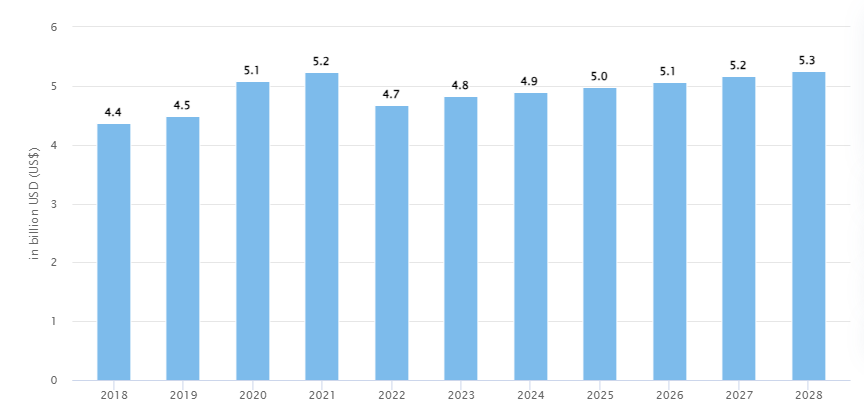
\includegraphics[width=1\textwidth]{imagenes/Capitulos/Cap12/RevenueKeyboardsWW.png}
    \caption{Ganancia global del mercado de teclados mecanicos \cite{Comercial1}.}
    \label{fig:RevenueWW}
\end{figure}

Actualmente, el mercado de teclados personalizados y de lujo se encuentra en una fase de crecimiento. La innovación constante y la introducción de nuevas tecnologías, como los teclados sin plate y las pantallas LED integradas, están impulsando la demanda y atrayendo a un número creciente de entusiastas de la tecnología y profesionales \ref{fig:VolumenWW}.

\begin{figure}[H]
    \centering
    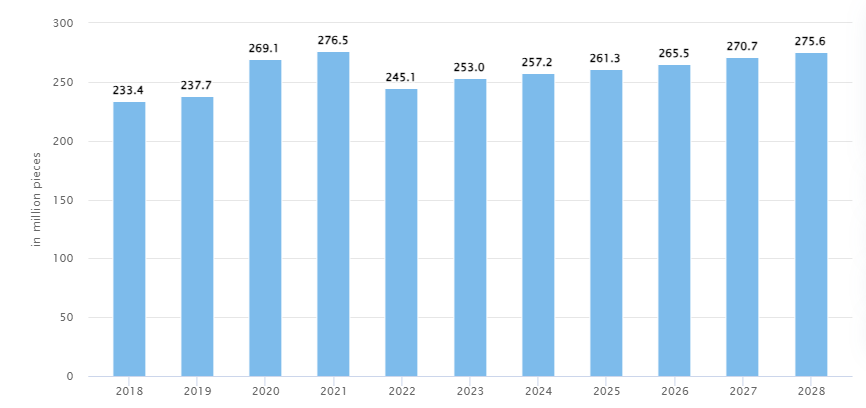
\includegraphics[width=1\textwidth]{imagenes/Capitulos/Cap12/VolumenKeyboard.png}
    \caption{Volumen global del mercado de teclados mecanicos \cite{Comercial1}.}
    \label{fig:VolumenWW}
\end{figure}

\subsubsection{Clientes}

Los clientes potenciales para este teclado incluyen:

\begin{itemize}
    \item \textbf{Gamers:} Buscan teclados con alta respuesta y personalización.
    \item \textbf{Profesionales de oficina:} Valoran la ergonomía y la durabilidad del teclado.
    \item \textbf{Entusiastas de la tecnología:} Interesados en productos innovadores y personalizables.
    \item \textbf{Consumidores de productos de lujo:} Buscan exclusividad y alta calidad.
\end{itemize}

\subsubsection{Proveedores}

Para la fabricación del teclado, se trabajará con proveedores de componentes electrónicos, materiales de alta calidad y servicios de fresado. Se han encontrado proveedores a muy bajo coste tanto para minoristas y mayoristas. Para los componentes electronicos tendriamos la empresa LCSC y junto con su filial JLCPCB para la fabricación de PCBs. 
Para los materiales de alta calidad se ha encontrado la empresa Keyreative que ofrece keycaps de alta calidad y personalizables. 
Para los servicios de fresado se ha encontrado empresas locales que ofrecen servicios de fresado a bajo coste. 
Para toda la logistica y distribución se ha encontrado la empresa DHL O GLS que ofrece servicios de envio a nivel mundial a precios competitivos.

\subsubsection{Estrategia}

Dando que seria necesario un gran capital para poder fabricar los teclados en masa, se ha decidido que la mejor estrategia seria la de fabricar los teclados bajo demanda. De esta manera se podria ofrecer un producto de alta calidad y personalizable a un precio competitivo. Además de no tener que tener un gran almacen con gran stock. Esto tambien abaratara los costes de produccion y almacenamiento. La estrategia más viable para este caso seria usar paginas de founding como Kickstarter o Indiegogo para poder financiar la producción de los teclados asi como para poder medir la demanda del producto y poder ajustar la producción a la demanda.

\subsubsection{Previsiones futuras}

Se espera que la demanda de teclados personalizados y de alta gama continúe creciendo en los próximos años. Las tendencias indican una preferencia creciente por productos que combinan funcionalidad, personalización y diseño exclusivo. Además, la expansión del mercado \textit{DIY} y el aumento del teletrabajo seguirán impulsando esta demanda.

\subsection{Análisis FODA}

\subsubsection{Fortalezas}

\begin{itemize}
    \item \textbf{Calidad y durabilidad:} Uso de materiales premium y diseño robusto.
    \item \textbf{Personalización:} Opciones de interruptores y keycaps intercambiables.
    \item \textbf{Innovación:} Diseño sin plate y pantalla LED integrada.
    \item \textbf{Exclusividad:} Producto fabricado a mano, único para cada usuario.
\end{itemize}

\subsubsection{Oportunidades}

\begin{itemize}
    \item \textbf{Crecimiento del mercado:} Aumento de la demanda de productos de lujo y personalizados.
    \item \textbf{Expansión geográfica:} Potencial para llegar a mercados internacionales.
    \item \textbf{Nuevas tecnologías:} Incorporación de innovaciones tecnológicas adicionales.
\end{itemize}

\subsubsection{Debilidades}

\begin{itemize}
    \item \textbf{Costo elevado:} El precio total de 249,54 \euro~puede ser una barrera para algunos consumidores.
    \item \textbf{Tiempo de fabricación:} Producción artesanal puede ser más lenta comparada con métodos industriales.
\end{itemize}

\subsubsection{Amenazas}

\begin{itemize}
    \item \textbf{Competencia:} Otros fabricantes de teclados personalizados y de alta gama.
    \item \textbf{Cambios en las tendencias de consumo:} Preferencias de los consumidores pueden cambiar.
\end{itemize}

\section{Costos, legal, marketing}

Un apartado importante para la viabilidad comercial de un producto es el análisis de los costos asociados con su producción, comercialización y distribución. Además, es necesario considerar los aspectos legales y de marketing para asegurar el cumplimiento de las regulaciones y la promoción efectiva del producto en el mercado.

\subsection{Costos}

Todos los costes por unidad vienen detallados en la tablas \ref{Table:ComponentesMontaje}, \ref{Table:ComponetesElectronicos}, \ref{Table:ServiciosHerramientas}. A estos costes habria que sumarle los costes de logistica y distribución. Además de los de marketing y publicidad. Aunque estos al ser costes variables no se pueden calcular con exactitud. Y dependerian bastante de la demanda del producto que se haria a partir de la campaña de founding. Por lo que se ha decidido no incluirlos en el calculo de los costes.

\subsubsection{Costos de producción} \label{SeccionCostosProduccion}

Dado que estos costos han sido calculados por unidad sin tener en cuenta la cantidad y sin tener en cuenta las ganancias. Facilmente podemos usar este precio de referencia para los siguientes calculos. El coste por unidad es de 249,54 \euro. Este precio incluye todos los componentes y servicios necesarios para la fabricación del teclado. (Estos podrian llegar a ser menor al aumentar la cantidad de unidades fabricadas).

\subsubsection{Costos de comercialización}

Los costos de comercialización incluyen todos los gastos necesarios para llevar el producto al mercado y hacerlo llegar a los consumidores. Estos costos pueden incluir:

\begin{itemize}
    \item \textbf{Publicidad:} Gastos en campañas publicitarias, tanto online como offline.
    \item \textbf{Promoción:} Descuentos, ofertas especiales y actividades promocionales.
    \item \textbf{Distribución:} Costos asociados al envío y manejo del producto.
    \item \textbf{Plataformas de venta:} Comisiones y tarifas de plataformas de venta online.
    \item \textbf{Marketing digital:} Costos de SEO, SEM, redes sociales y marketing de contenidos.
\end{itemize}

Para estimar los costos de comercialización, se considera un porcentaje del precio de venta. En este caso, se estima que los costos de comercialización representan aproximadamente el 20\% del precio de venta. Este porcentaje sigue un razonamiento basado en la naturaleza del producto, los canales de comercialización y competencia en el mercado. Y por supuesto basado en ejemplos de productos similares en el mercado.

\subsubsection{Calculo del costo de comercialización}
Se ha investigado y se han encontrado ejemplos de productos similares en plataformas de venta como Amazon, Etsy, y tiendas especializadas. Estas plataformas suelen implicar comisiones que varían entre el 10\% y el 15\% del precio de venta. Comparando con productos similares en la industria tecnológica, especialmente aquellos de nicho y personalizados, es común asignar entre un 15\% y un 25\% del precio de venta a los costos de comercialización. Este rango permite cubrir adecuadamente todos los aspectos necesarios para lanzar y mantener un producto en el mercado.

Por lo tanto, se ha estimado que un 20\% del precio de venta es un valor razonable para los costos de comercialización. Este porcentaje no comprometerá la viabilidad del proyecto, ya que la estrategia a seguir es de financiación bajo demanda.

\begin{equation}
\text{Costo de comercialización} = 0,20 \times 249,54 \euro = 49.91 \euro
\end{equation}

\subsubsection{Costos de administración}
Ya que este proyecto lo estaria llevando a cabo yo solo, y los costes asociados al personal ya estan incluidos en los costes de producción. No habria costes adicionales asociados a la administración.

\subsubsection{Costos de financiamiento}
Como la estrategia elegida es la de financiación bajo demanda, no habria costes asociados a financiamiento. Ya que el capital necesario para la producción del teclado se obtendria a traves de la campaña de founding y vendria de los propios clientes, estos pagarian por adelantado el producto.

Aunque Kickstarter e Indiegogo cobran una comisión por el uso de sus plataformas, esta comisión se deduce directamente del dinero recaudado y es del 5\% en Kickstarter \cite{ComisionKickStarer} y de maximo 8\% en Indiegogo \cite{ComisionIndiegogo}. Por lo que no se considera un coste adicional.

\subsubsection{Costos de impuestos}

Los costos de impuestos incluyen todos los tributos que la empresa debe pagar, tales como:

\begin{itemize}
    \item \textbf{Impuesto sobre la renta:} Impuesto sobre las ganancias de la empresa.
    \item \textbf{Impuesto al valor agregado (IVA):} Impuesto sobre las ventas de productos.
    \item \textbf{Contribuciones sociales:} Impuestos relacionados con los empleados. (No aplicable en este caso)
\end{itemize}

Dado que el iva en España es del 21\% \cite{IVA}, el coste de impuestos seria de y el impuesto sobre la renta es del 24\% \cite{ImpuestoRenta}, el coste de impuestos seria de:

\begin{equation}
    \text{Costo de impuestos} = 0,21 \times 249,54 \euro + 0,24 \times 249,54 \euro = 112.29 \euro
\end{equation}

\subsection{Total de costos}
Computando todos los costes, el coste total por unidad seria de:

\begin{equation}
    \text{Costo total} = 249,54 \euro + 49,91 \euro + 112,29 \euro = 411,74 \euro
\end{equation}

Este sería el precio máximo que se podría vender el teclado sin tener en cuenta las ganancias. Aunque este precio podría ser menor al aumentar la cantidad de unidades fabricadas, llegaría a poder disminuirse hasta un 35\% para más de 1000 unidades fabricadas y de 30\% para más de 500 unidades fabricadas.
El precio total de coste de una unidad sería de 411,74 \euro.
El precio total de coste de 100 unidades sería de 337.63 \euro.
El precio total de coste de 500 unidades sería de 288.22 \euro.
El precio total de coste de 1000 unidades sería de 267.63 \euro.

\subsection{Aspectos legales}

La consideración de los aspectos legales es fundamental para asegurar que el negocio del teclado fabricado a mano opere dentro del marco legal adecuado y proteja sus activos intelectuales. A continuación, se describen los pasos necesarios para cumplir con las regulaciones legales y proteger la propiedad intelectual del producto.

\subsubsection{Registro de la empresa}

Para asegurar que el capital personal no corra peligro, se recomienda establecer la empresa como una \textbf{Sociedad de Responsabilidad Limitada (S.L.)}, donde los socios no responden personalmente por las deudas sociales, sino únicamente con el capital aportado.

\textbf{Proceso jurídico para darse de alta en el Registro Mercantil:}

\begin{enumerate}
    \item \textbf{Certificación negativa del nombre:} Solicitar una certificación negativa del nombre de la sociedad en el Registro Mercantil Central para asegurarse de que el nombre elegido no esté ya registrado.
    \item \textbf{Redacción de los estatutos sociales:} Elaborar los estatutos sociales que regirán la empresa. Estos deben incluir la denominación social, el objeto social, el domicilio social, el capital social y la estructura de administración de la sociedad.
    \item \textbf{Apertura de una cuenta bancaria:} Depositar el capital social mínimo (3.000 euros) en una cuenta bancaria a nombre de la futura sociedad. El banco emitirá un certificado del depósito.
    \item \textbf{Otorgamiento de la escritura pública:} Acudir a una notaría para otorgar la escritura pública de constitución de la sociedad, que debe incluir la certificación negativa del nombre, los estatutos sociales y el certificado del banco.
    \item \textbf{Obtención del Número de Identificación Fiscal (NIF) provisional:} Solicitar el NIF provisional en la Agencia Tributaria, presentando la escritura de constitución y el modelo 036 de alta censal.
    \item \textbf{Inscripción en el Registro Mercantil:} Presentar la escritura pública de constitución en el Registro Mercantil de la provincia donde la empresa tendrá su domicilio social. Una vez inscrita, la sociedad adquirirá plena personalidad jurídica.
    \item \textbf{Obtención del NIF definitivo:} Con la inscripción en el Registro Mercantil, se debe acudir nuevamente a la Agencia Tributaria para obtener el NIF definitivo.
    \item \textbf{Alta en el Impuesto de Actividades Económicas (IAE):} Registrar la empresa en el IAE, obligatorio para realizar actividades comerciales en España.
\end{enumerate}

\subsubsection{Registro de la marca}

El registro de la marca es crucial para proteger el nombre y el logotipo del teclado. Los pasos incluyen:

\begin{enumerate}
    \item \textbf{Búsqueda de antecedentes:} Realizar una búsqueda para asegurarse de que la marca no esté ya registrada por otra empresa.
    \item \textbf{Solicitud de registro:} Presentar una solicitud de registro ante la Oficina Española de Patentes y Marcas (OEPM).
    \item \textbf{Revisión y publicación:} La OEPM revisará la solicitud y, si no hay objeciones, publicará la marca en el Boletín Oficial de la Propiedad Industrial (BOPI).
    \item \textbf{Registro internacional:} Considerar el registro internacional de la marca si se planea expandir el mercado fuera de España, utilizando el Sistema de Madrid de la Organización Mundial de la Propiedad Intelectual (OMPI).
\end{enumerate}

\subsubsection{Registro de la patente}

Si el teclado incorpora innovaciones técnicas únicas, puede ser necesario patentar esas innovaciones:

\begin{enumerate}
    \item \textbf{Preparación de la solicitud:} Documentar detalladamente la innovación técnica, incluyendo dibujos y descripciones técnicas.
    \item \textbf{Presentación de la solicitud:} Presentar la solicitud de patente ante la OEPM.
    \item \textbf{Examen de fondo:} La OEPM realizará un examen de fondo para evaluar la novedad y la aplicabilidad industrial de la invención.
    \item \textbf{Concesión de la patente:} Si la solicitud es aprobada, se concede la patente, que proporciona protección legal durante un periodo de 20 años.
\end{enumerate}

\subsubsection{Registro de derechos de autor}

Para proteger el software y otros elementos creativos del teclado, se debe considerar el registro de derechos de autor:

\begin{enumerate}
    \item \textbf{Documentación:} Compilar toda la documentación necesaria que demuestre la autoría y la originalidad del software y otros elementos creativos.
    \item \textbf{Presentación de la solicitud:} Registrar los derechos de autor en el Registro de la Propiedad Intelectual, presentando la documentación requerida.
    \item \textbf{Certificación:} Obtener el certificado de registro, que provee evidencia legal de la autoría y la fecha de creación.
\end{enumerate}

\subsubsection{Registro de licencias}

Dependiendo de la naturaleza del negocio, puede ser necesario obtener varias licencias:

\begin{enumerate}
    \item \textbf{Licencias comerciales:} Licencias necesarias para operar el negocio, incluyendo licencias municipales si se va a tener un establecimiento físico.
    \item \textbf{Licencias de software:} Si se utiliza software de terceros en el desarrollo del teclado, es crucial asegurarse de que se cuenta con las licencias adecuadas.
    \item \textbf{Licencias medioambientales:} Si el proceso de fabricación implica el uso de materiales o procesos que pueden tener un impacto medioambiental, se debe obtener las licencias correspondientes.
\end{enumerate}

\textbf{Conclusión}

Cumplir con los aspectos legales es fundamental para proteger el negocio y asegurar su funcionamiento dentro del marco regulatorio. La correcta implementación de estos pasos ayudará a minimizar riesgos legales y a proteger los activos intelectuales de la empresa.


\subsection{Marketing}

El marketing es una parte crucial del éxito de cualquier producto en el mercado. Para el teclado fabricado a mano, se han diseñado estrategias específicas para aumentar su visibilidad, atraer a clientes potenciales y asegurar una distribución efectiva.

\subsubsection{Estrategias de marketing}

Las estrategias de marketing se centran en destacar las características únicas del teclado y en llegar al público objetivo. Estas incluyen:

\begin{itemize}
    \item \textbf{Segmentación de mercado:} Identificar y centrarse en los segmentos de mercado que valoran la personalización, la calidad y la innovación en teclados, como los entusiastas de la tecnología, los gamers y los profesionales creativos.
    \item \textbf{Posicionamiento de marca:} Posicionar el teclado como un producto de lujo y \textit{DIY}, destacando su diseño personalizado, la calidad de los materiales y la exclusividad.
    \item \textbf{Estrategia de diferenciación:} Resaltar las características únicas del teclado, como su diseño sin plate, la pantalla LED y la personalización completa de \textit{keycaps} e interruptores.
    \item \textbf{Marketing digital:} Utilizar las redes sociales, el SEO y el marketing de contenido para aumentar la visibilidad del teclado en línea y atraer tráfico al sitio web de ventas.
\end{itemize}

\subsubsection{Publicidad}

La publicidad se enfocará en aumentar la notoriedad del teclado y atraer a clientes potenciales a través de diferentes medios:

\begin{itemize}
    \item \textbf{Redes sociales:} Utilizar plataformas como Instagram, Facebook y Twitter para mostrar fotos y videos del teclado, resaltar sus características únicas y compartir contenido generado por los usuarios.
    \item \textbf{Anuncios en línea:} Implementar campañas de anuncios pagados en Google Ads y redes sociales para dirigir tráfico al sitio web de ventas.
    \item \textbf{Colaboraciones con influenciadores:} Trabajar con influenciadores en el ámbito de la tecnología y los videojuegos para promover el teclado a sus seguidores.
    \item \textbf{Publicidad en medios especializados:} Publicar anuncios en revistas y sitios web especializados en tecnología y hardware de computadora.
\end{itemize}

\subsubsection{Promoción}

Las promociones incentivarán las compras y aumentarán la fidelidad del cliente:

\begin{itemize}
    \item \textbf{Descuentos por lanzamiento:} Ofrecer descuentos especiales durante el lanzamiento del teclado para atraer a los primeros compradores.
    \item \textbf{Programas de referidos:} Incentivar a los clientes actuales a referir a nuevos clientes a través de descuentos y recompensas.
    \item \textbf{Ofertas por tiempo limitado:} Crear ofertas especiales por tiempo limitado para incentivar compras rápidas.
    \item \textbf{Regalos promocionales:} Incluir regalos promocionales como herramientas de personalización de teclados o fundas protectoras con cada compra.
\end{itemize}

\subsubsection{Distribución}

La distribución eficiente asegura que los teclados lleguen a los clientes de manera rápida y segura:

\begin{itemize}
    \item \textbf{Ventas en línea:} Principalmente a través de un sitio web propio y plataformas de comercio electrónico como Amazon y Etsy.
    \item \textbf{Logística y envío:} Asociarse con empresas de logística confiables para asegurar tiempos de envío rápidos y seguros tanto a nivel nacional como internacional.
    \item \textbf{Almacenamiento:} Mantener un inventario adecuado para satisfacer la demanda y evitar retrasos en los envíos.
\end{itemize}

\subsubsection{Ventas}

Las estrategias de ventas se centrarán en convertir a los visitantes del sitio web y a los seguidores en clientes:

\begin{itemize}
    \item \textbf{E-commerce optimizado:} Asegurar que el sitio web de ventas sea fácil de navegar, seguro y optimizado para conversiones.
    \item \textbf{Servicio al cliente:} Ofrecer un excelente servicio al cliente, incluyendo soporte en tiempo real, garantías y políticas de devolución claras.
    \item \textbf{Contenido educativo:} Proporcionar contenido educativo sobre el montaje y la personalización del teclado para ayudar a los clientes a tomar decisiones informadas.
\end{itemize}

\subsubsection{Alianzas estratégicas}

Las alianzas estratégicas pueden ayudar a expandir el alcance del teclado y mejorar su oferta:

\begin{itemize}
    \item \textbf{Colaboraciones con fabricantes de componentes:} Trabajar con fabricantes de \textit{keycaps}, interruptores y otros componentes para asegurar la calidad y obtener precios competitivos.
    \item \textbf{Socios de distribución:} Formar alianzas con minoristas y plataformas de venta en línea para aumentar la visibilidad y las ventas del teclado.
    \item \textbf{Eventos y ferias:} Participar en eventos y ferias de tecnología para mostrar el teclado a un público más amplio y establecer relaciones comerciales.
\end{itemize}

\textbf{Conclusión}

El desarrollo y la implementación de una estrategia de marketing integral es esencial para el éxito del teclado fabricado a mano. Estas estrategias ayudarán a posicionar el producto en el mercado, aumentar su visibilidad y asegurar un flujo constante de clientes satisfechos.
